Analiza el siguiente texto y responde a las preguntas:

\begin{boxE}
    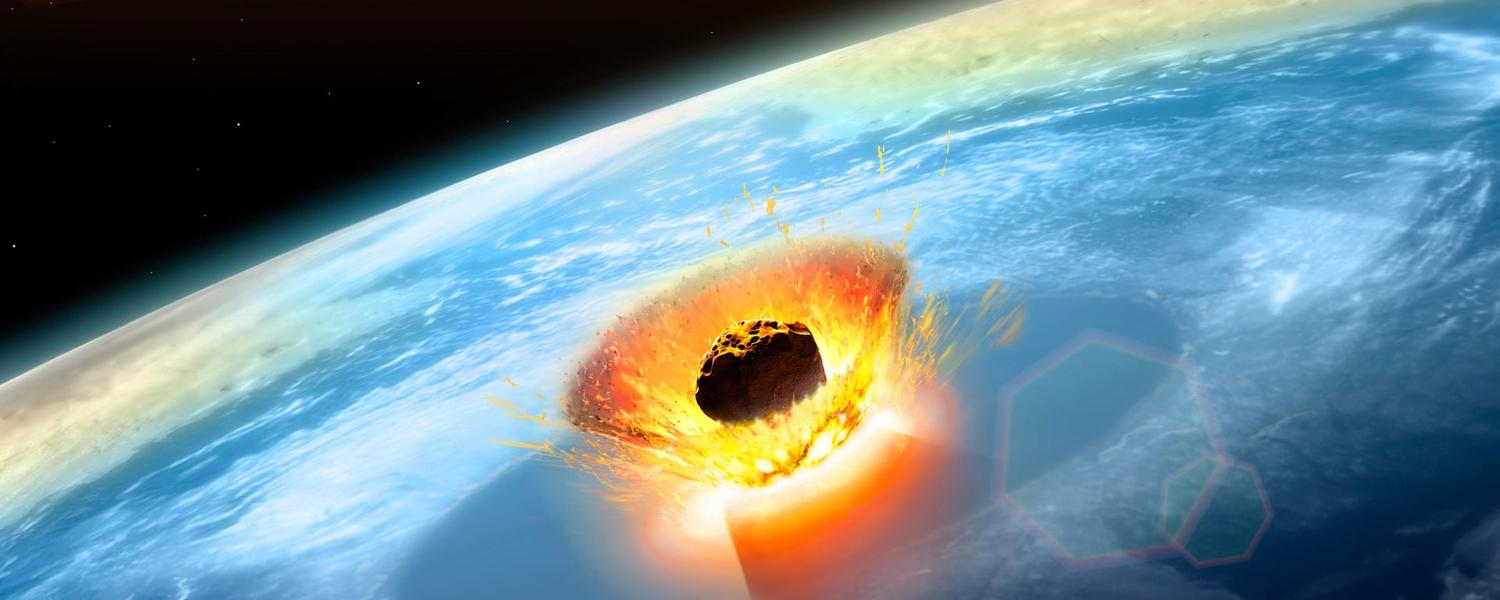
\includegraphics[width=\linewidth]{../images/5582.jpg}
    ¿Conoces la teoría del meteorito que causó la extinción de los dinosaurios
    hace 65 millones de años? Los científicos dicen que cayó sobre la península
    de Yucatán y que la energía del impacto era equivalente a la que liberarían
    5,000 millones de bombas atómicas como la lanzada sobre Nagasaki. El
    meteorito debió tener un diámetro mayor a 10 km y moverse a $54,000$ km/h.
    Debido al impacto se formó un cráter de 100 km de diámetro, se elevó
    la temperatura en esa zona y se produjo un enorme resplandor: fragmentos
    incandescentes, tanto del meteorito como del terreno donde cayó, salieron
    disparados provocando incendios en distintas partes del planeta.
    Como consecuencia del choque se levantó una gran cantidad de polvo
    que cubrió el cielo e impidió el paso de la luz solar, lo que limitó la fotosíntesis de las plantas y alteró las redes tróficas.
\end{boxE}

\begin{parts}
    \include*{../parts/question002a}
    \include*{../parts/question002b}
    \include*{../parts/question002c}
\end{parts}
